\section{Strided and Offset Memory Access (3 Points)}

\subsection{Task a}
In figure \ref{task_1_a_plot} it can be observed that strided memory access has a negative
impact on the effective memory bandwidth, the more the data are strided. A recommenddation
could be, to try to omit strided mermoy access and more try to access data in blocks which
are contiguous by design.

\begin{figure}[h]
    \begin{center}
        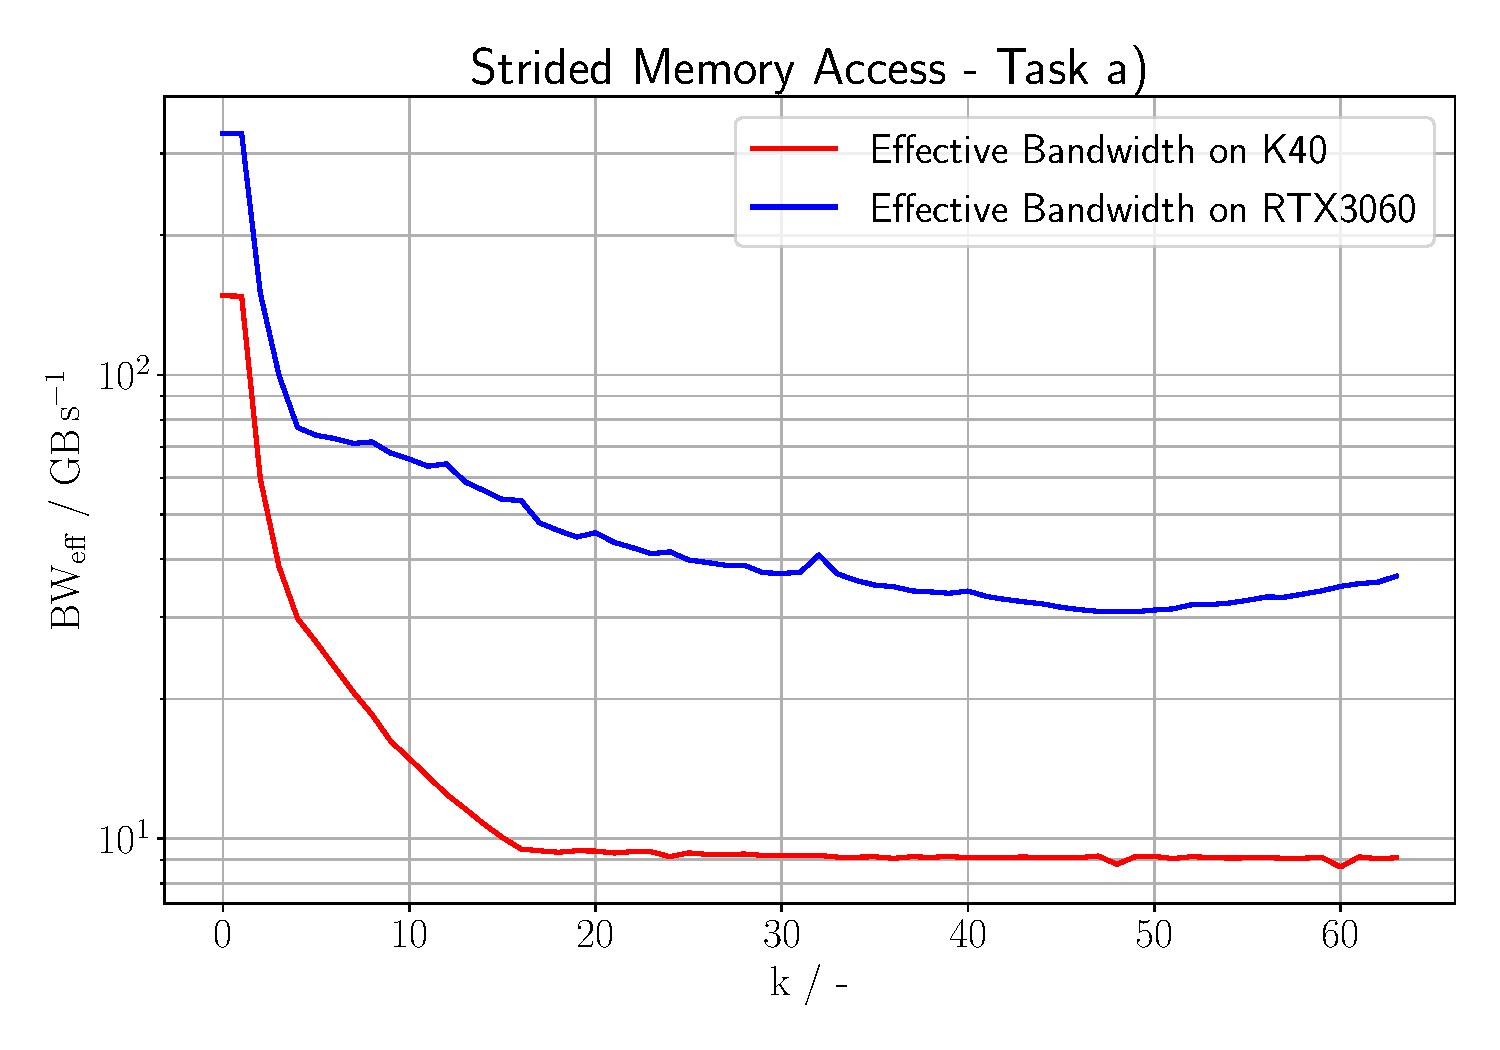
\includegraphics[width=1\textwidth]{figures/task_1_a.pdf}
        \caption{Plot for task 1a - see code in appendix \ref{app_1a}}
        \label{task_1_a_plot}
    \end{center}
\end{figure}
\pagebreak

\subsection{Task b}
In figure \ref{task_1_b_plot}, it can be observed that the effective memory bandwidth is 
always around the maximal bandwidth and has its peaks for $ \mathrm{k} \, \mathrm{mod}(4) = 0$
since sizes of this pattern fit better in \texttt{<<<256,256>>>}.
\begin{figure}[h]
    \begin{center}
        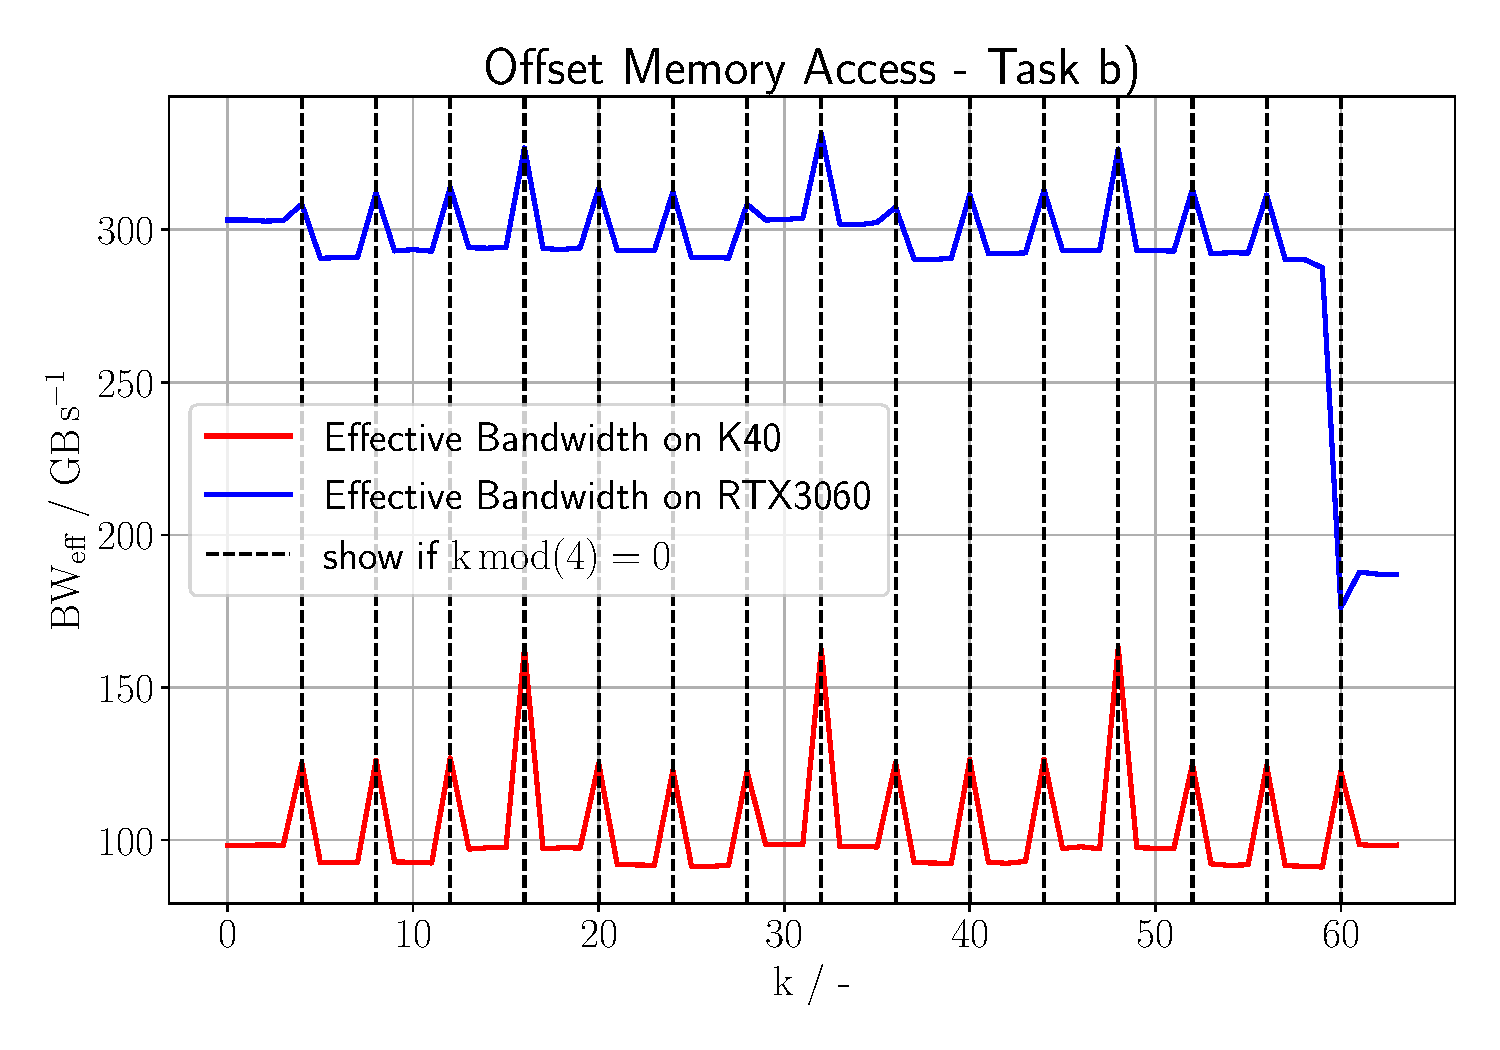
\includegraphics[width=1\textwidth]{figures/task_1_b.pdf}
        \caption{Plot for task 1b - see code in appendix \ref{app_1b}}
        \label{task_1_b_plot}
    \end{center}
\end{figure} 
\pagebreak


\section{Dense Matrix Transpose (6 Points)}
\subsection{Task a}
The implementation of my friend yields a memory leakage of 800 bytes in one allocation
because the allocated memory is not free'd after the program has finished. Additionally, 
the implementation does not yield correct results for aribtrary matrix dimensions.

\begin{lstlisting}[language=python, title=Console Output on RTX3060 Environment for transpose.cu]
$> timeout 30s cuda-memcheck --tool memcheck --leak-check full ./1a404f09.out 2>&1

0, 1, 2, 3, 4, 5, 6, 7, 8, 9,
.
.
.
90, 91, 92, 93, 94, 95, 96, 97, 98, 99,

Time for transpose: 0.00088
Effective bandwidth: 0.00181818 GB/sec

0, 10, 20, 30, 40, 50, 60, 70, 80, 90,
.
.
.
9, 19, 29, 39, 49, 59, 69, 79, 89, 99,
========= CUDA-MEMCHECK
========= Leaked 800 bytes at 0x7efd1c600000
=========     Saved host backtrace up to driver entry point at cudaMalloc time
=========     Host Frame:/lib/x86_64-linux-gnu/libcuda.so.1 [0x292c27]
=========     Host Frame:./1a404f09.out [0x30e03]
=========     Host Frame:./1a404f09.out [0xc3db]
=========     Host Frame:./1a404f09.out [0x41a7f]
=========     Host Frame:./1a404f09.out [0x81b2]
=========     Host Frame:./1a404f09.out (main + 0xae) [0x7c9f]
=========     Host Frame:/lib/x86_64-linux-gnu/libc.so.6 (__libc_start_main + 0xf3) [0x24083]
=========     Host Frame:./1a404f09.out (_start + 0x2e) [0x7a6e]
=========
========= LEAK SUMMARY: 800 bytes leaked in 1 allocations
========= ERROR SUMMARY: 1 error
\end{lstlisting}

\pagebreak

\subsection{Task b}
In order to be able to transpose arbitrarily sized matrices the kernel arguments
need to be adapted. See Appendix \ref{app_2b} line 63, where the the argument
$<<<(N+255) / 256, 256>>>$ is changed to $<<<(N^2+255) / 256, 256>>>$. The effective 
Bandwidth of the fixed Kernel is 0.00182025 GB/sec.

\subsection{Task c}
In Task c the in-place requirement is dropped, this is done by adapting the Kernel
in the following way:

\begin{lstlisting}[language=C++, title=C++ Listing for EX2 c Kernel Part]
__global__
void transpose(double *A, double *B, int N)
{
  int t_idx = blockIdx.x*blockDim.x + threadIdx.x;
  int row_idx = t_idx / N;
  int col_idx = t_idx % N;
  
  if (row_idx < N && col_idx < N) B[row_idx * N + col_idx] = A[col_idx * N + row_idx];
}
\end{lstlisting}

Also one needs to initialize device and host variables of the same size for the B matrix
and one mustn't forget to free the additional memory afterwards. See code in appendix
\ref{app_2b}.



